%% This is an example first chapter.  You should put chapter/appendix that you
%% write into a separate file, and add a line \include{yourfilename} to
%% main.tex, where `yourfilename.tex' is the name of the chapter/appendix file.
%% You can process specific files by typing their names in at the 
%% \files=
%% prompt when you run the file main.tex through LaTeX.

\chapter{Introduction}

asdfdsf

\section{Related Work}

asdfdsf

\subsection{Macro Assembly}

kenny's paper, batmen stuff

\subsection{Micro Assembly}

\begin{figure}
  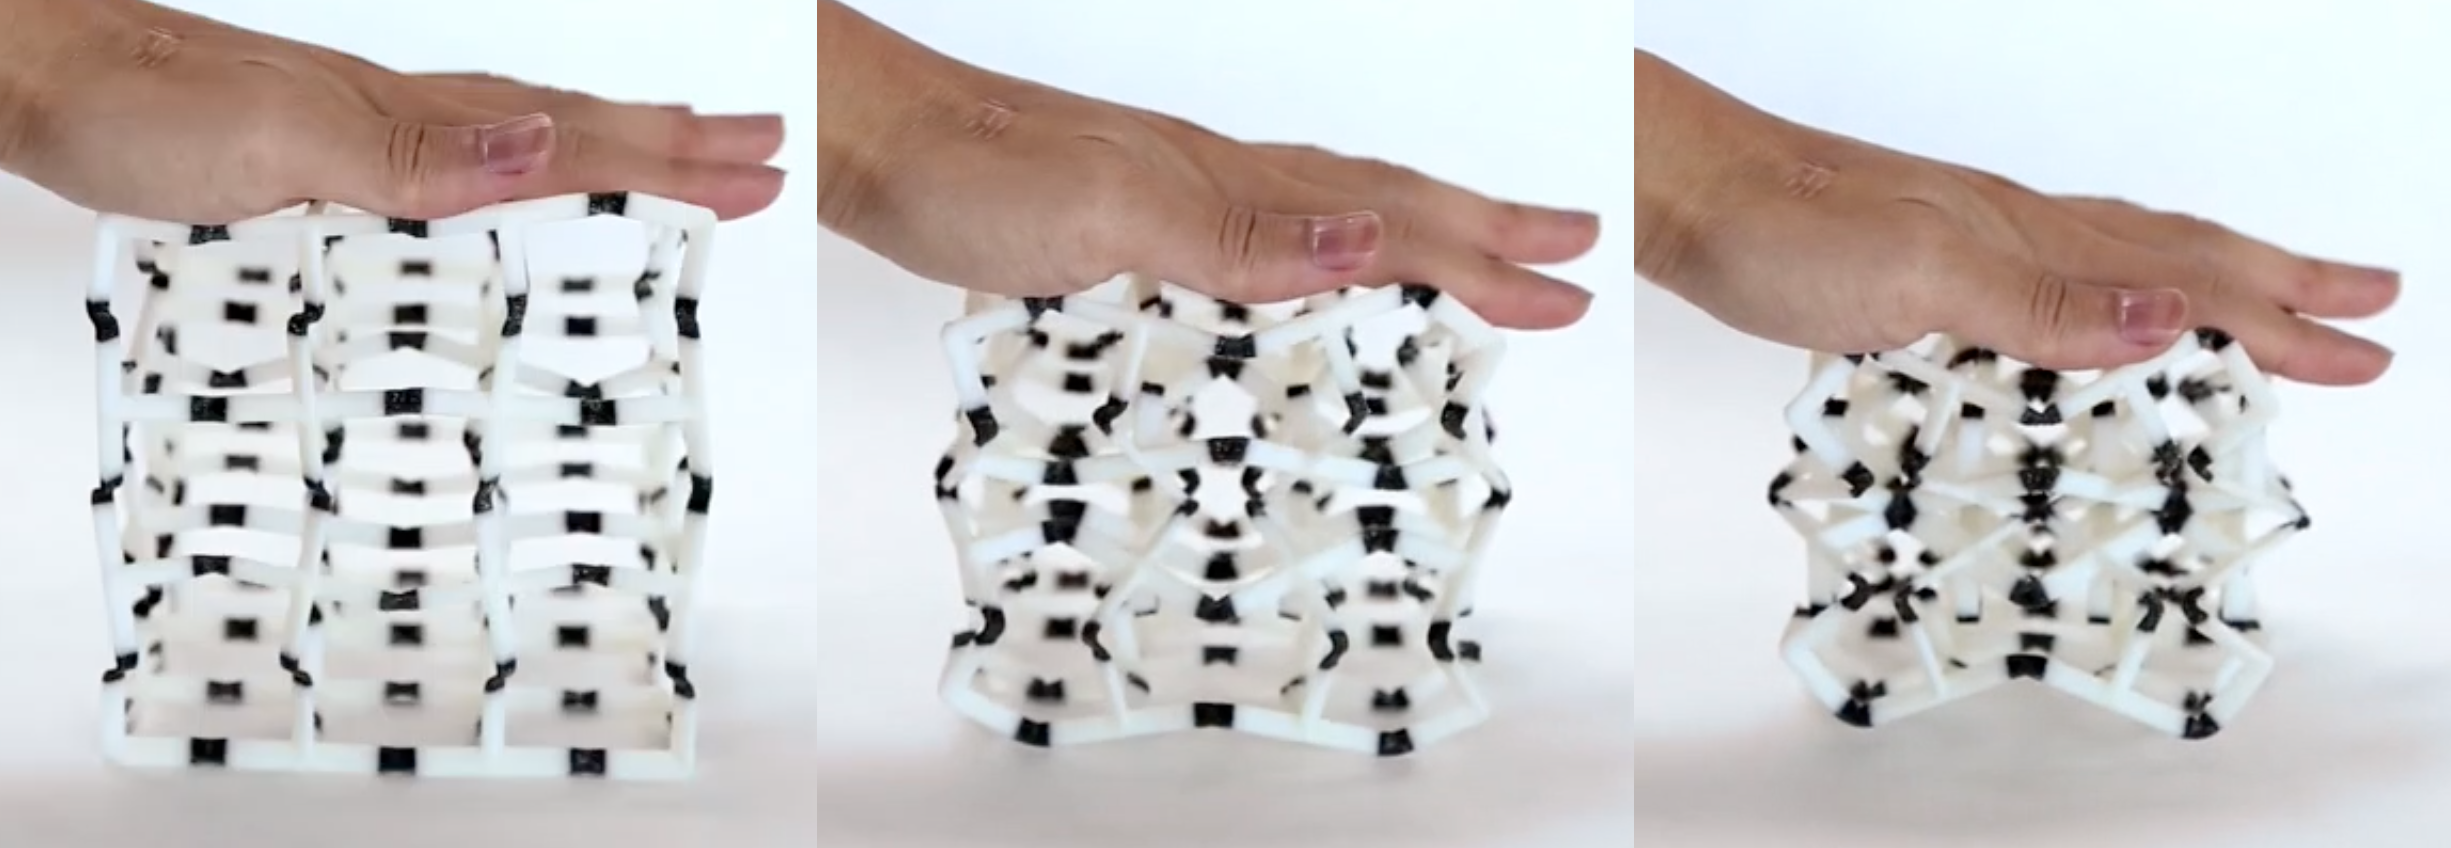
\includegraphics[width=\linewidth]{objetMultimaterial.png}
  \caption{Mechanical properties programmed by material deposition in Objet 3D print.}
  \label{fig: objetMultimaterial}
\end{figure}


Objet
Will - look at will's thesis to find other examples of discrete micro assembly

\subsection{Nano Assembly}

dna bricks, lithography

\subsection{CAD tools}

voxcad
voxel for multi material 3d printing
minecraft
conway's designer
other digital materials cad references?

\subsection{Simulation}

sam's stuff

\section{Proposed Work}

asdfdsf

\subsection{Design}

asdfdsf

\begin{figure}
  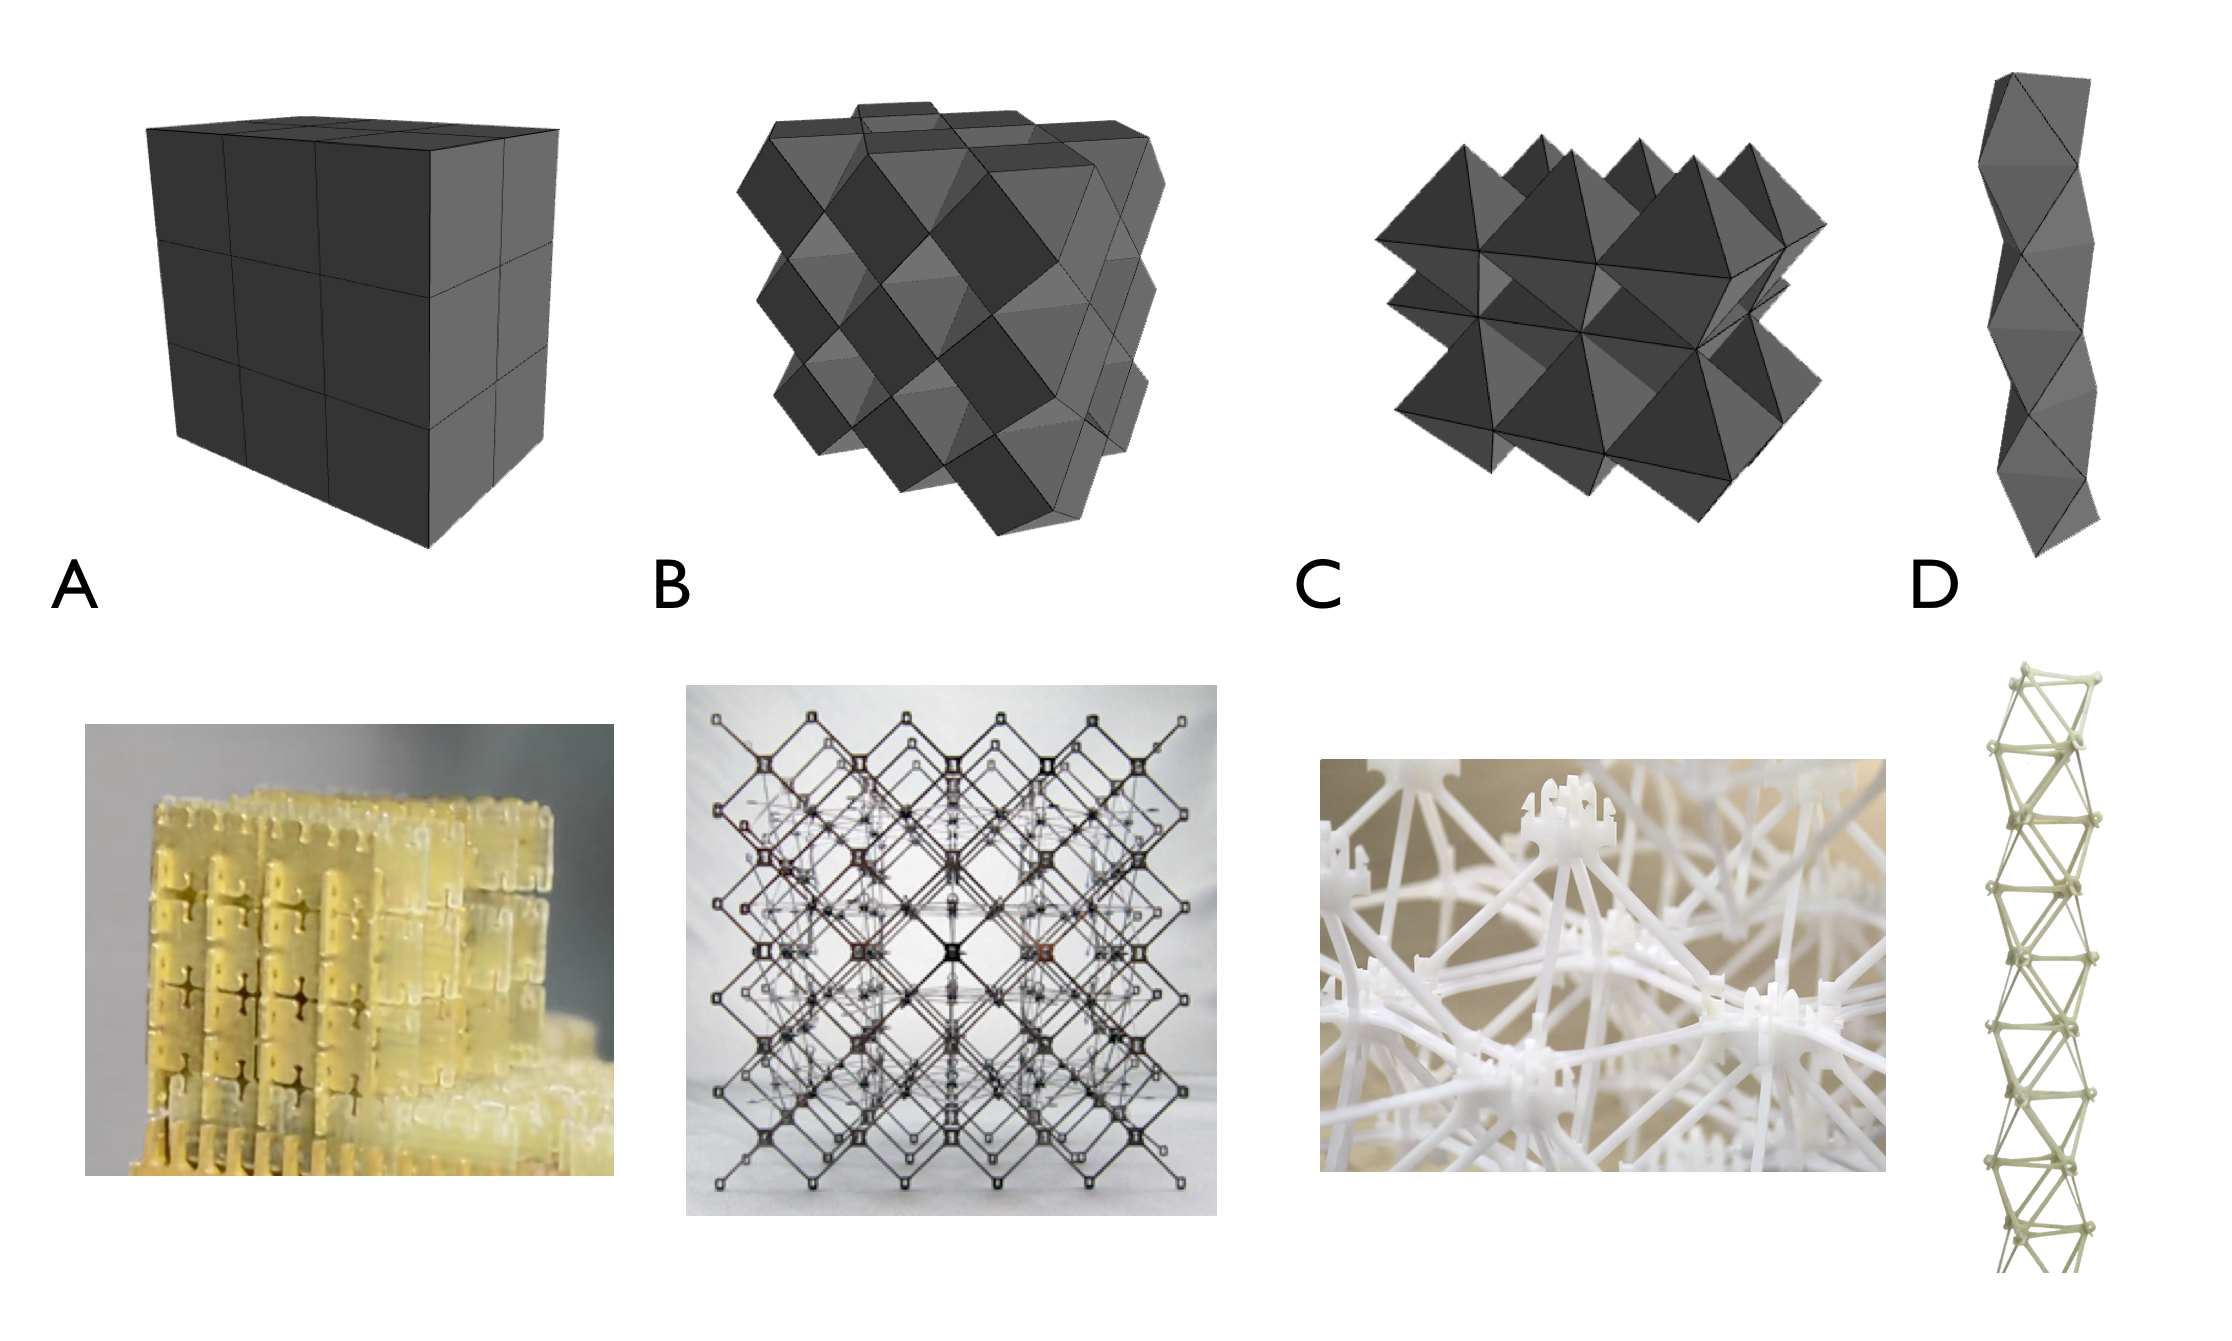
\includegraphics[width=\linewidth]{latticeVirtualRealComp.png}
  \caption{Comparison of virtual lattice types with their real world counterparts.}
  \label{fig: latticeVirtualRealComp}
\end{figure}

\begin{figure}
  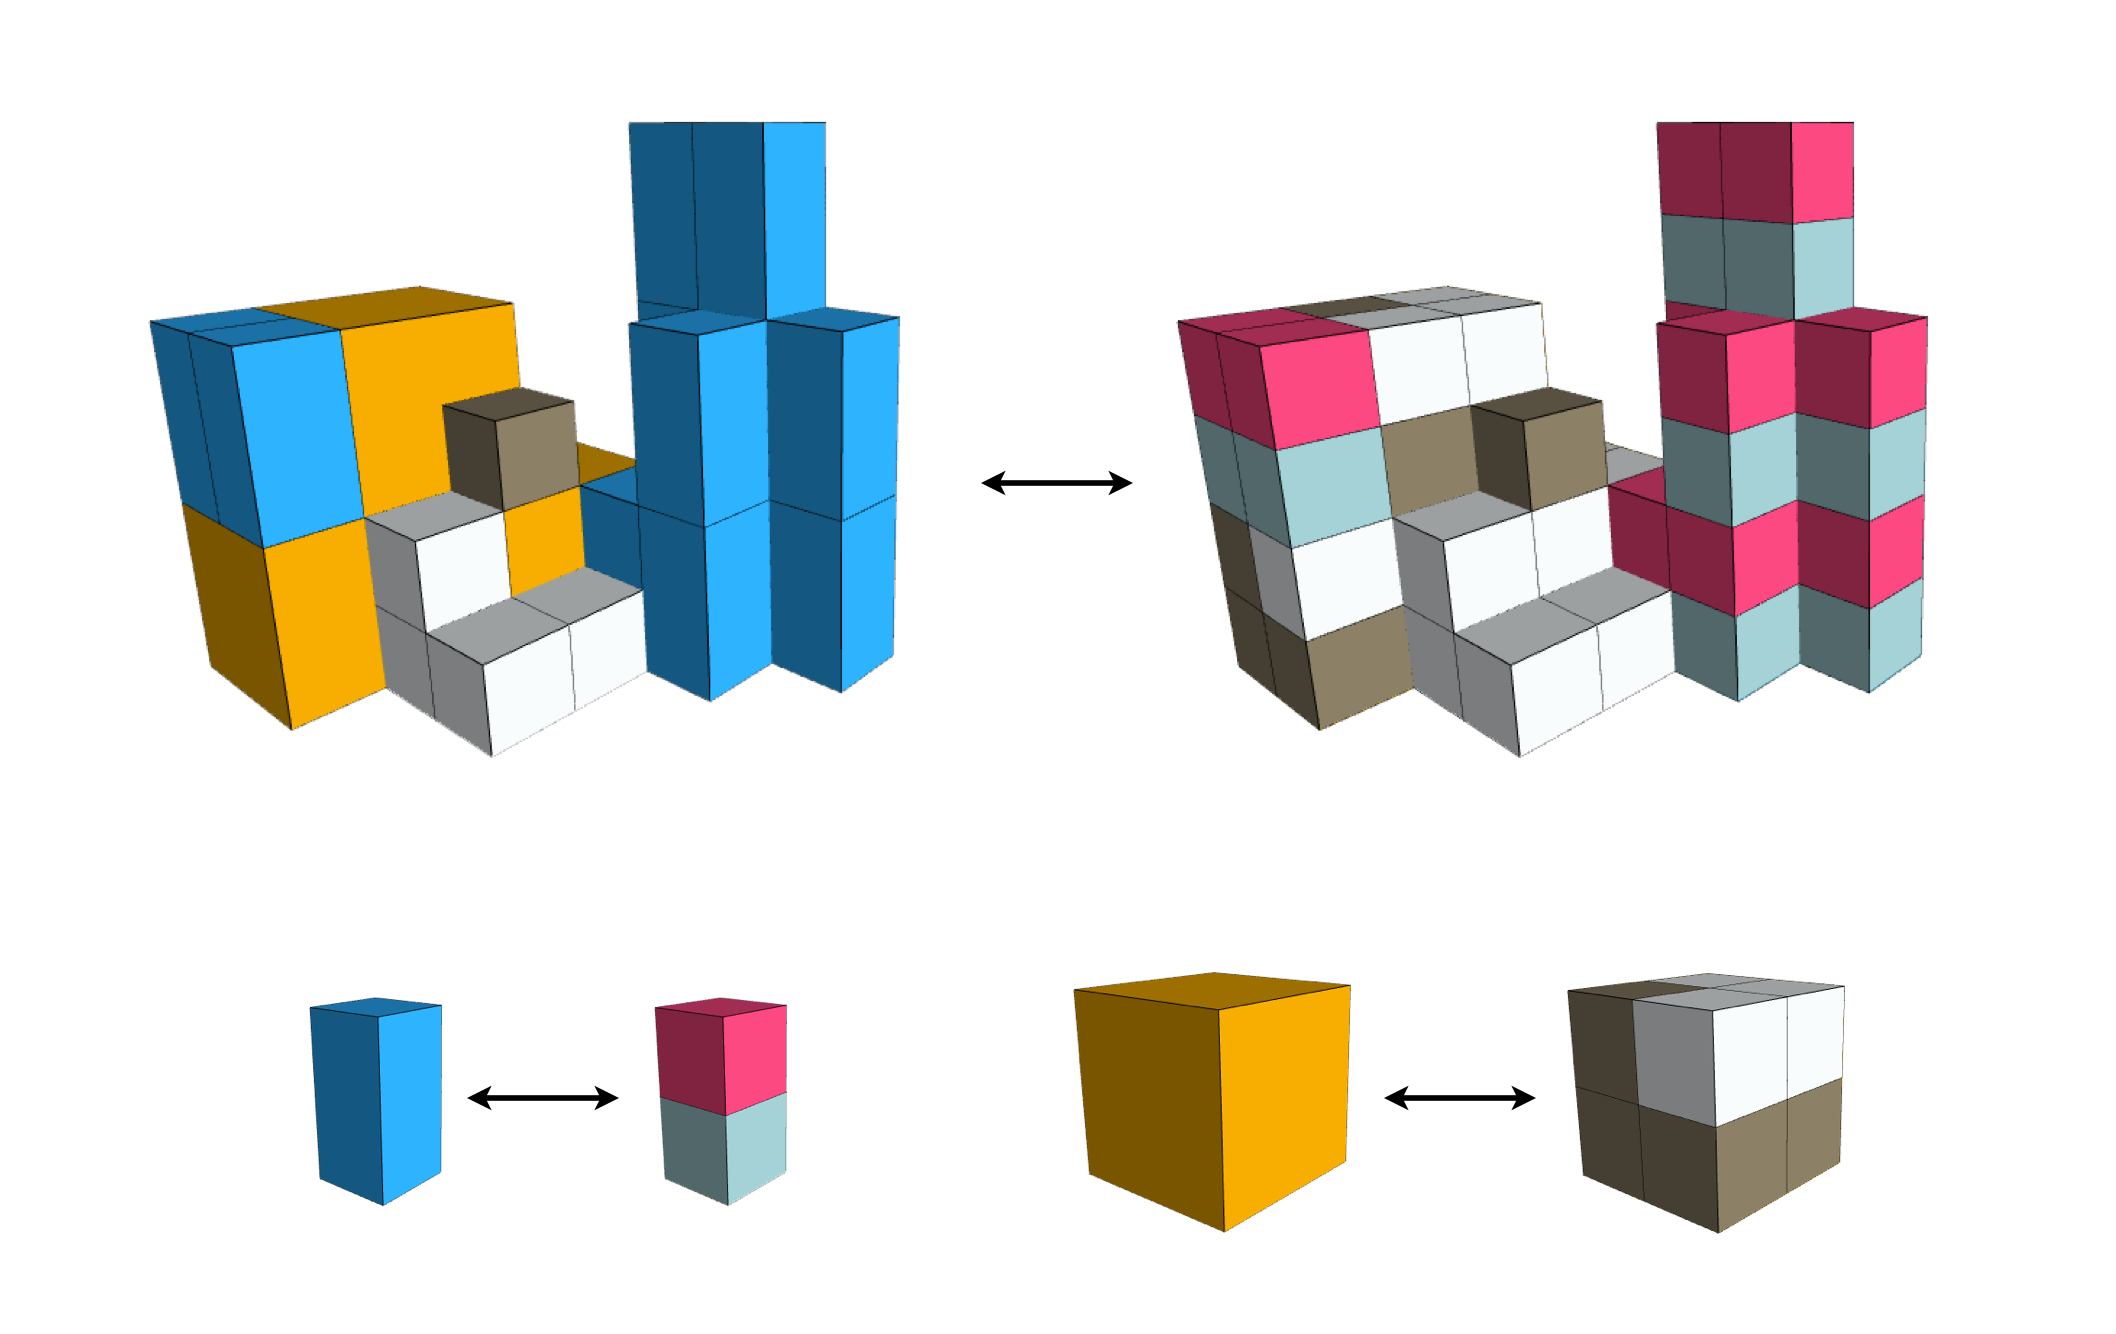
\includegraphics[width=\linewidth]{hierarchicalDecomp.png}
  \caption{Hierarchical decomposition of lattice assembly. All hierarchical components are parametrically linked to a hierarchical material definition.}
  \label{fig:hierarchicalDecomp}
\end{figure}

\begin{figure}
  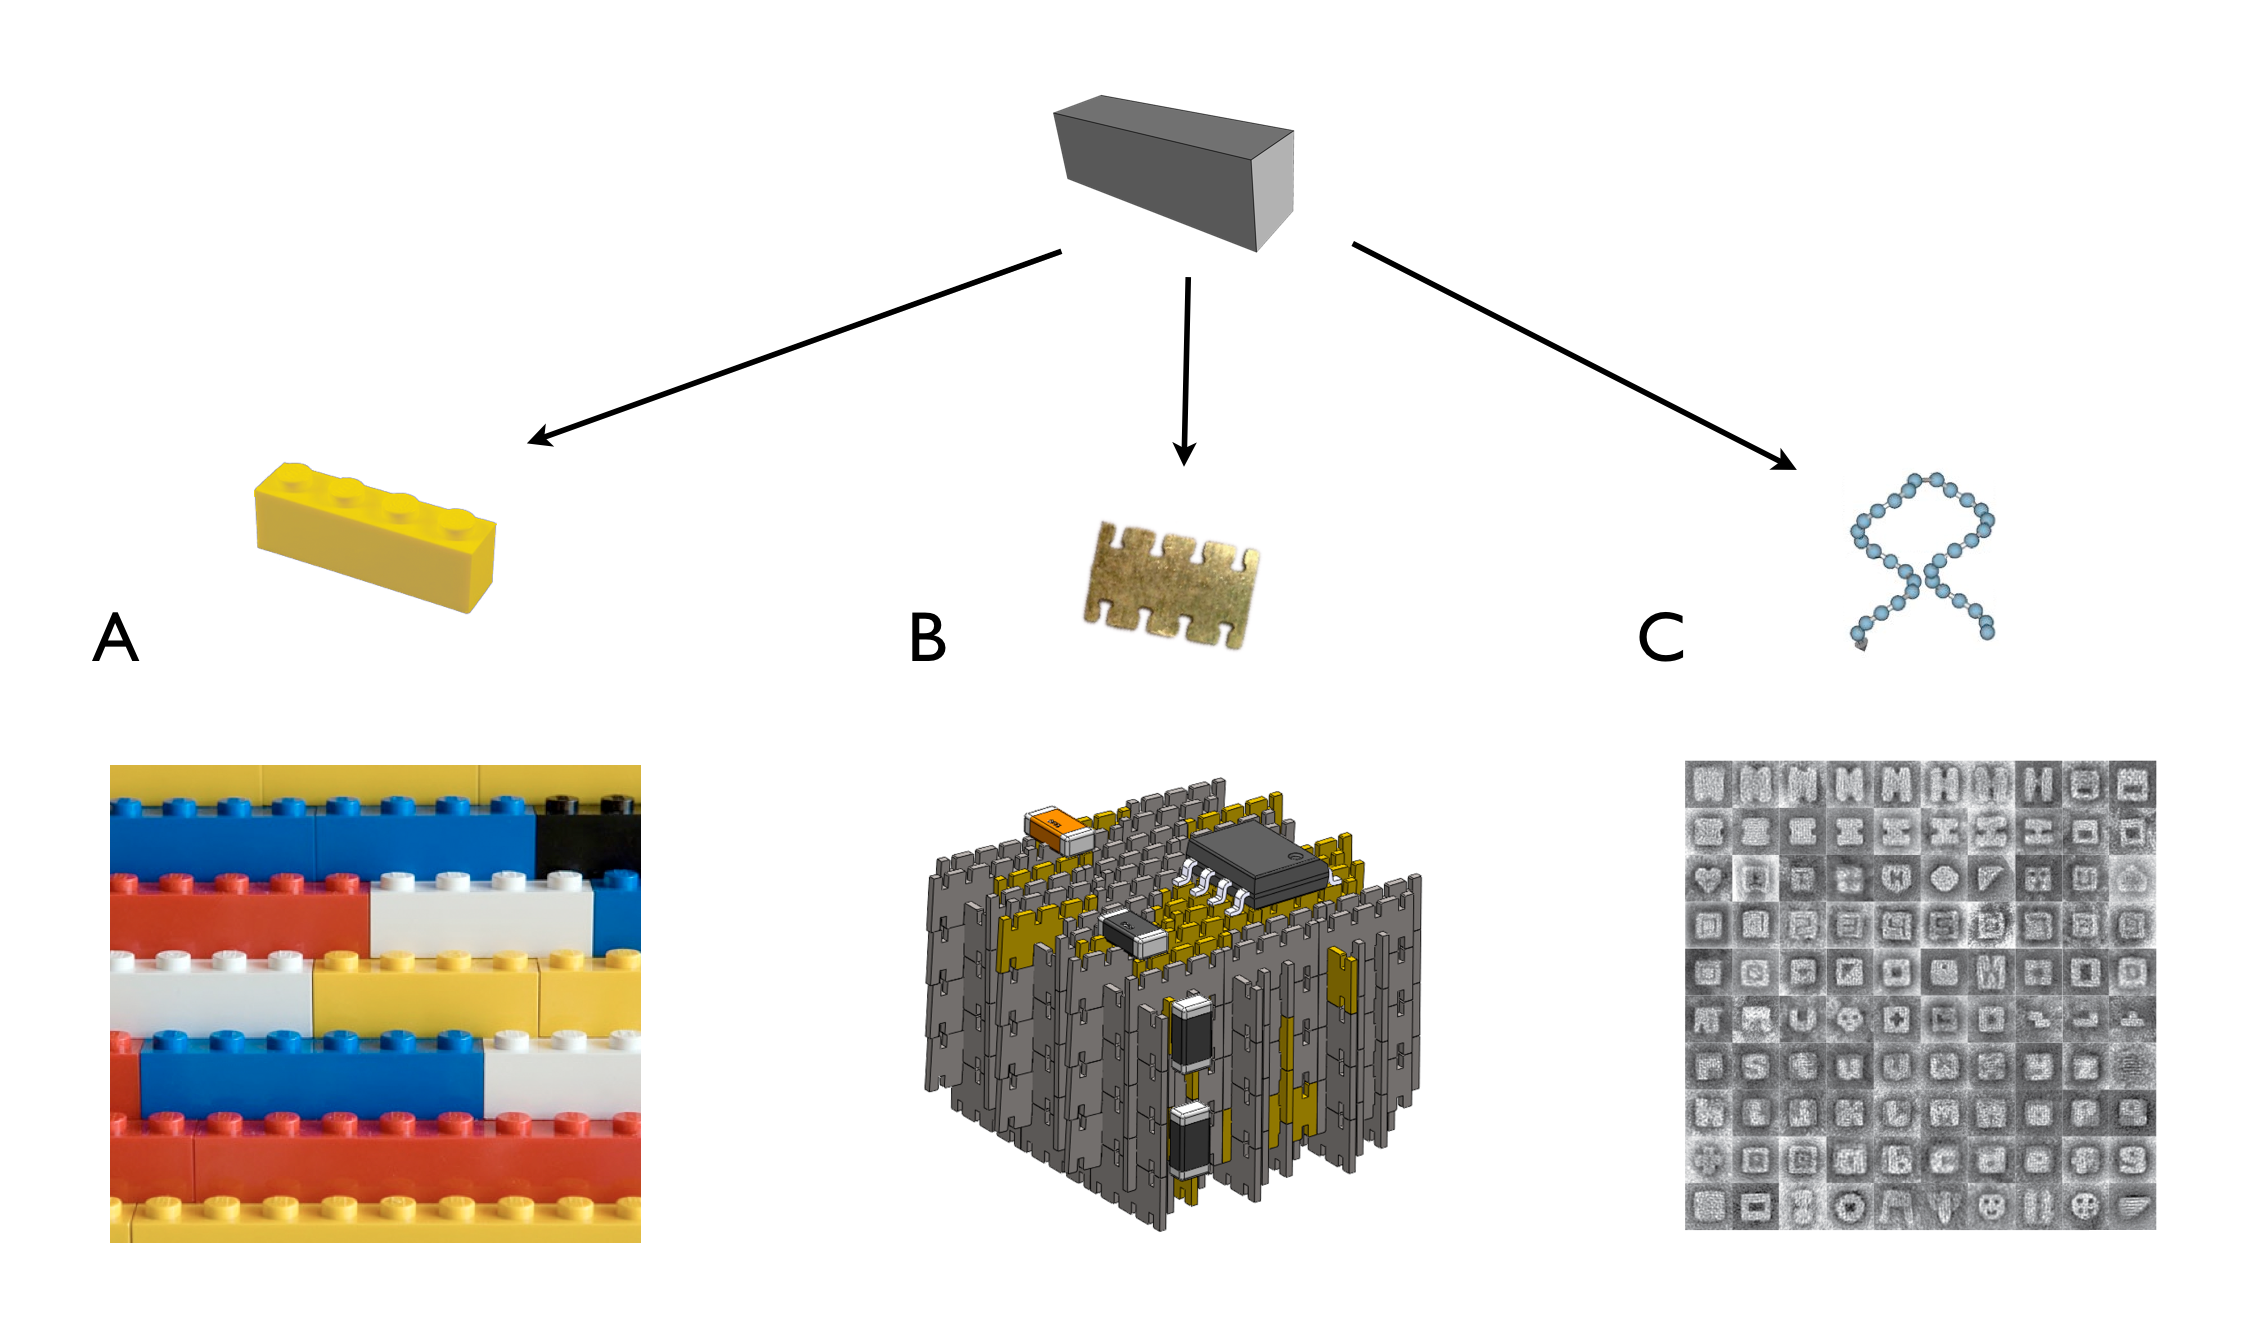
\includegraphics[width=\linewidth]{partAbstraction.png}
  \caption{Part abstraction from lattice primitive.}
  \label{fig: partAbstraction}
\end{figure}

\subsection{Simulation}

describe different realms of sim we're looking at currently
how to modularize?

\subsection{Assembly}

\begin{figure}
  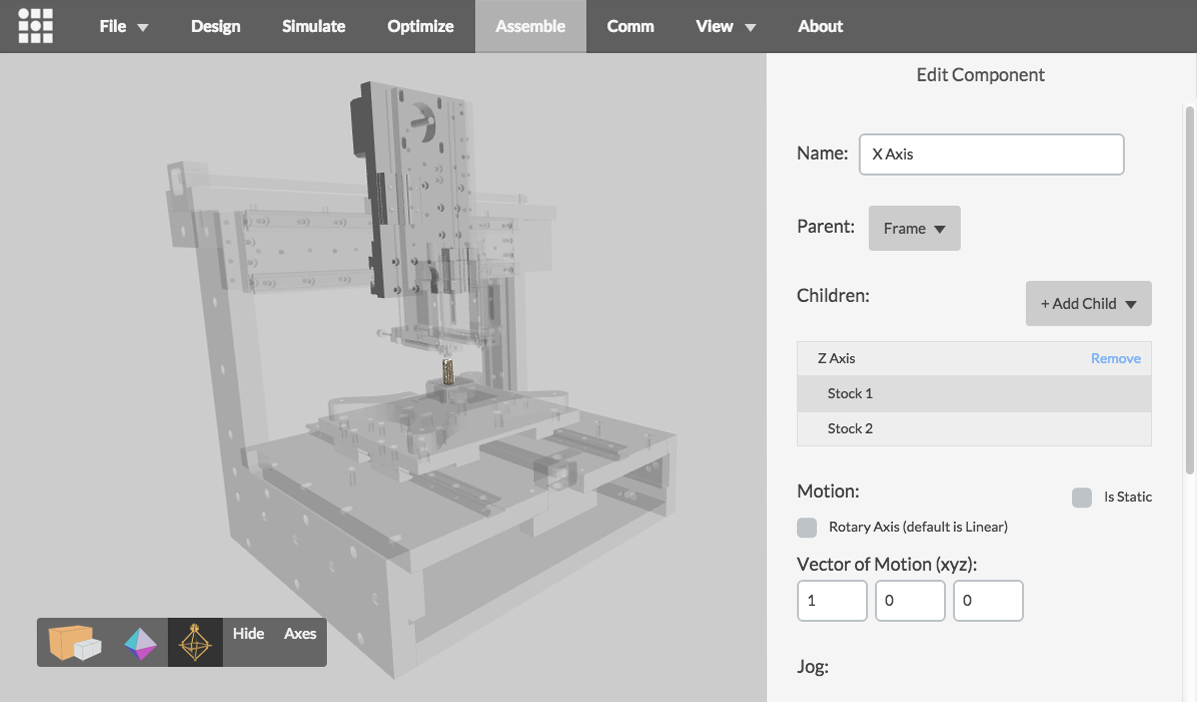
\includegraphics[width=\linewidth]{assemblerSetup1.png}
  \caption{Screenshot of current assembler config GUI.}
  \label{fig: assembleSetup1}
\end{figure}

\begin{figure}
  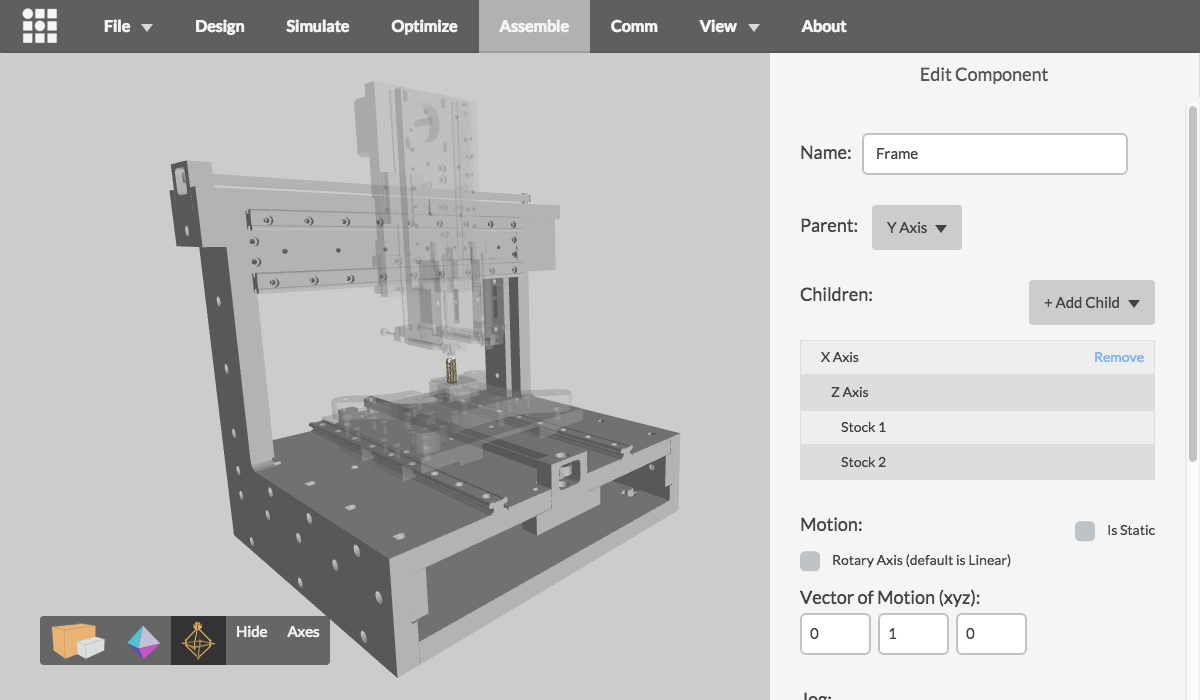
\includegraphics[width=\linewidth]{assemblerSetup2.png}
  \caption{Screenshot of current assembler config GUI.}
  \label{fig: assembleSetup2}
\end{figure}

urdf, tree description for abstraction
calculate reverse kinematics
abstraction of strategies and assemblers/low level operation

\subsection{GUI}

\begin{figure}
  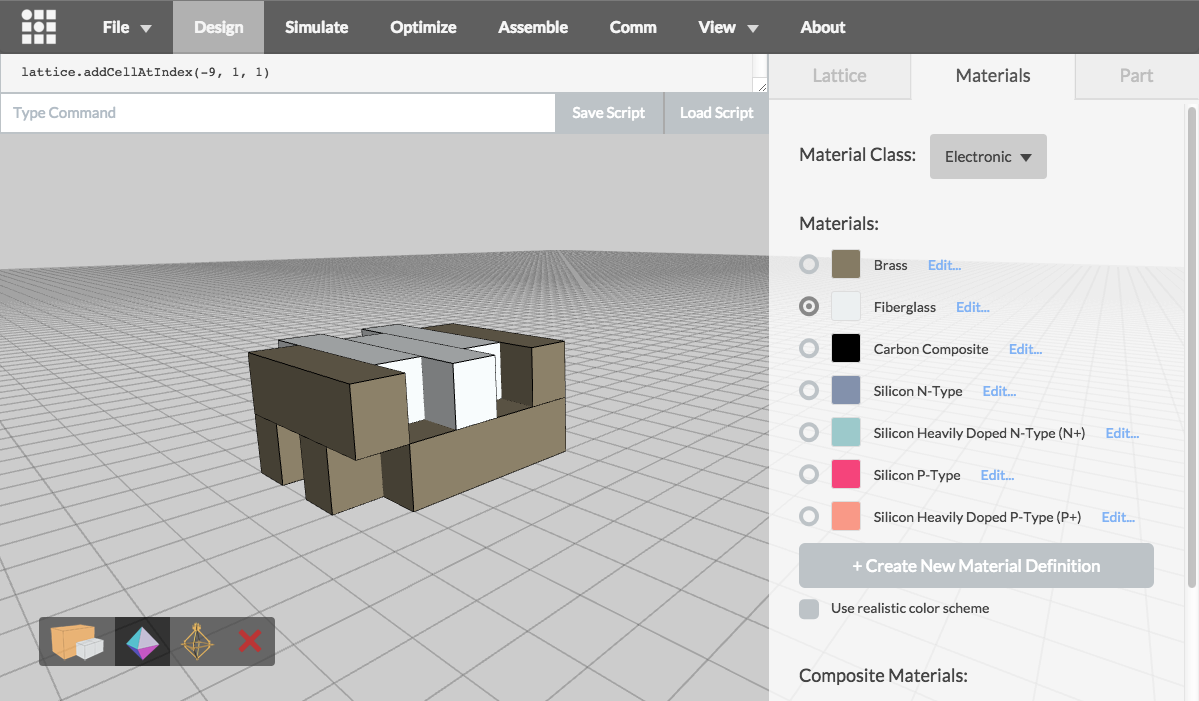
\includegraphics[width=\linewidth]{designGUI.png}
  \caption{Screenshot of current design GUI.}
  \label{fig: designGUI}
\end{figure}

\begin{figure}
  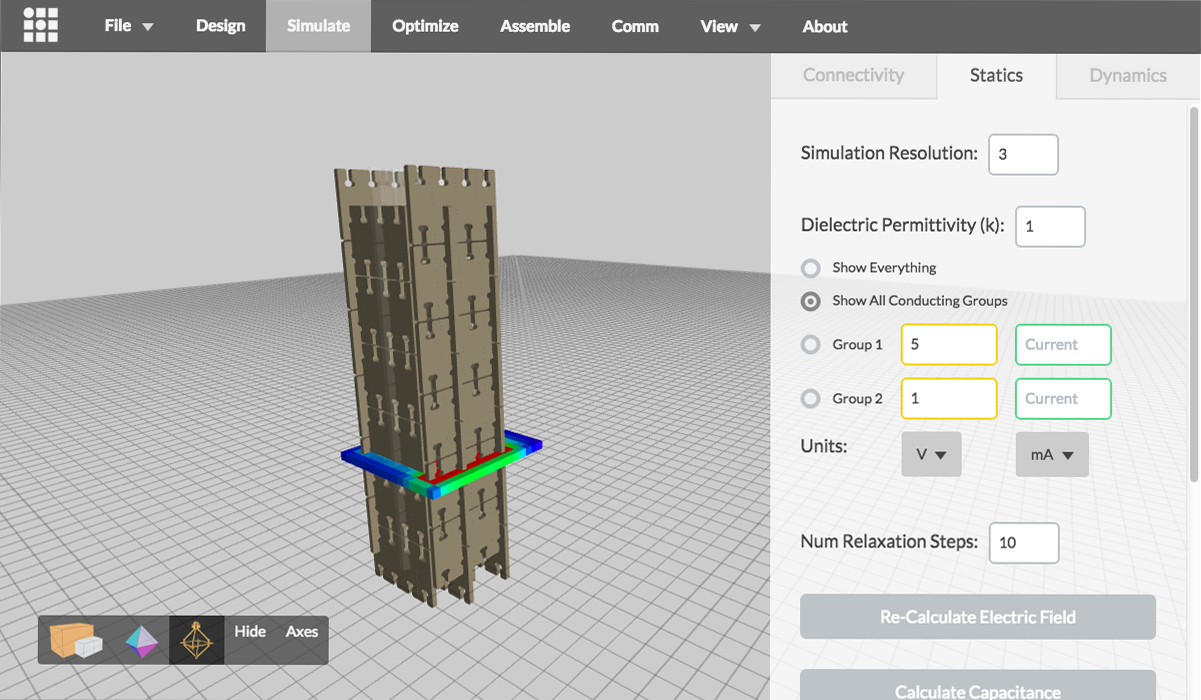
\includegraphics[width=\linewidth]{simGUI.png}
  \caption{Screenshot of current simulation GUI.}
  \label{fig: simGUI}
\end{figure}

\begin{figure}
  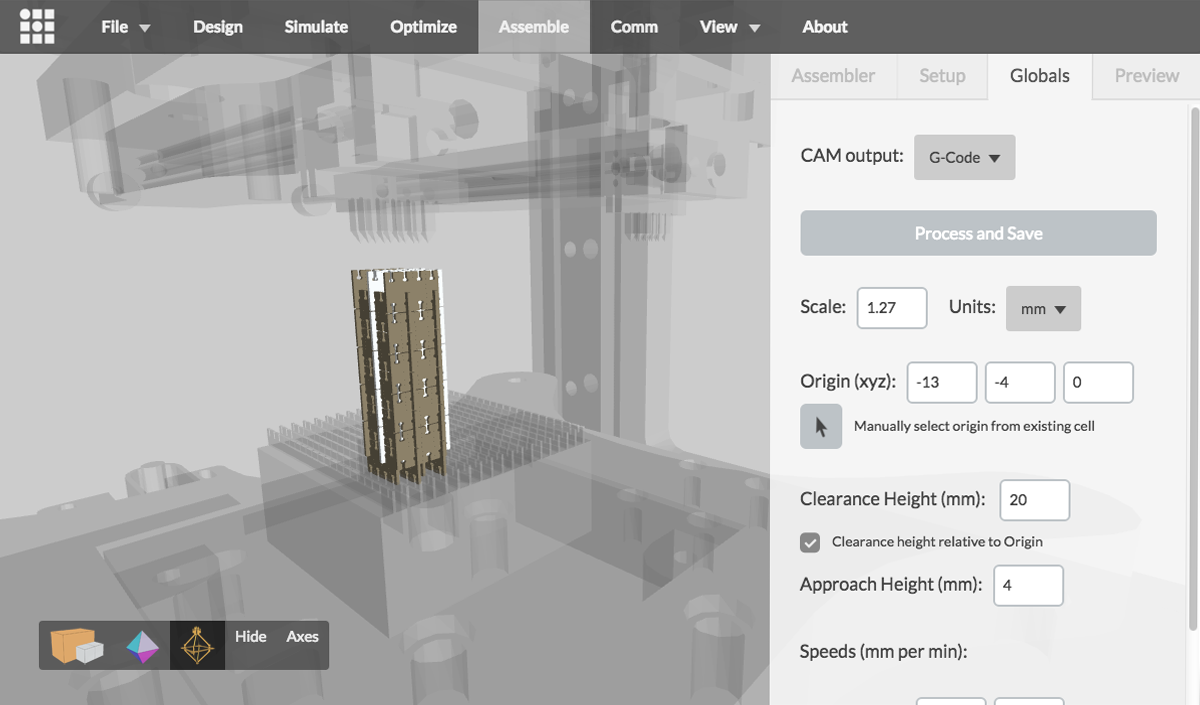
\includegraphics[width=\linewidth]{assembleGUI.png}
  \caption{Screenshot of current assemble GUI.}
  \label{fig: assembleGUI}
\end{figure}

javascript, etc, etc

\subsection{API}

Lattice, Cell, Material, CompositeMaterial classes.

\begin{figure}
  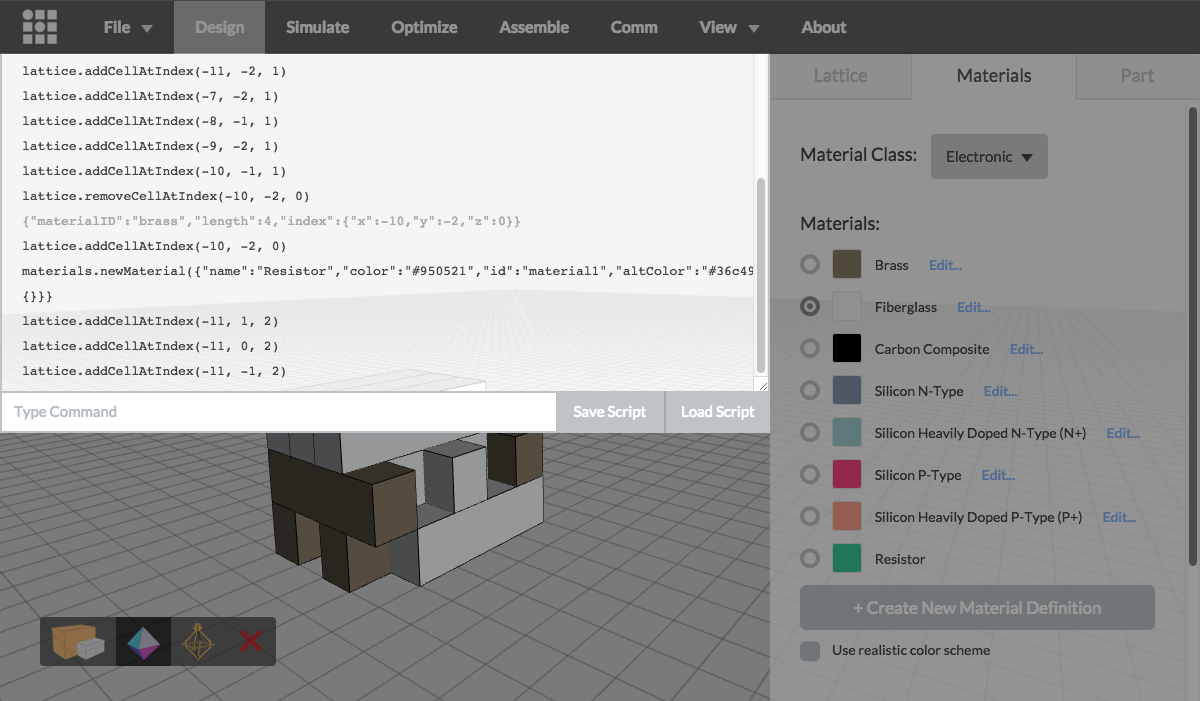
\includegraphics[width=\linewidth]{scriptGUI.png}
  \caption{Screenshot of current script GUI for API with scripting console highlighted.}
  \label{fig: scriptGUI}
\end{figure}

asdfdsf

\section{Contribution}

asdfdsf

\section{Evaluation}

asdfdsf

\section{Resources Required}

The majority of the work involved in this thesis will happen in the computer and require no material resources.  If required, I will use CBA's cluster for highly parallel computational operations.  Fabrication of assemblers and parts to be used in the digital assembler workflows should be considered outside the scope of material resources required by this thesis, and will be supplied by CBA.

\section{Schedule}

\begin{description}
  \item[11/6/15]\tabto{1.5cm}Proposal Due - main design classes and design API are nearly complete.  First pass at assembly workflow is complete.  Some aspects of electronics simulation have been started.
  \item[11/9/15]\tabto{1.5cm}Crit Day Presentation
  \item[11/15]\tabto{1.5cm}Meeting with potential Harvard collaborators to discuss ways to expand on the DNA assembly portion of the workflow.  Finishing touches on design workflow and API.  Users should now be able to create their own design scripts and upload them to the GUI (e.g. Will wants a script that fills in empty space around conducting elements with insulating elements.  He doesn't know it yet, but he's going to write that himself and upload it to the GUI).
  \item[12/15]\tabto{1.5cm}Refactor of assembler workflow for compatibility with URDF.  Planning for assembler API.
  \item[1/15]\tabto{1.5cm}I will spend January at NASA Ames to work with Kenny Cheung, Ben Jenett, and Daniel Cellucci on bringing in one of our new locomotion robots (Mojo) into my software workflow.  By this time I should have completed a refactor of the assembler tree code.  If successful, incorporating the new robot into my software will be accomplished entirely through the GUI, generating a config file that I can load into the codebase. 
  \item[2/15]\tabto{1.5cm}Finishing touches on assembler workflow and assembler API.  Add ability to load user scripts with assembly strategies (assembly strategies describe the order to add cells to the lattice).
  \item[3/15]\tabto{1.5cm}Linear FEA modeling of mechanical structures.
  \item[4/15]\tabto{1.5cm}
  \item[5/15]\tabto{1.5cm}
  \item[6/6]\tabto{1.5cm}Thesis Due
\end{description}
